\chapter{Environment}
\section{Foraging}
\subsection{Foraging Background}

Foraging is a base requirement that is needed as it is a method of obtaining more resources from the starting amount. Currently in the MVP foraging is based on the concept of inputting resources to get a return.\\

\subsubsection{Underlying concept}
The goal of foraging in this “game” is to introduce a certain dilemma to the agents to further understand the behaviours of multiple (6) intelligent agents working together to reach a goal with different personal goals. By having 2 methods of foraging it introduces the concept of decision making between the islands allowing for strategic interactions to maximise personal benefits whilst still reaching the overarching goal of survival.\\  

The inspiration for our concept of foraging comes from the stag hunt game furthermore it introduces elements from it. Specifically it brings in the concept of \textbf{no dominant strategy} and how \textbf{ one agents choice can impact other agents.}\\

The concept of stag hunt is that each player selects a method of hunting and if they differ then the social welfare (total payoff) is significantly less than if they both go stag hunting. The selection of stag means the agent is going for higher \textbf{payoff}whilst the selection of hare indicates that the agent is going for \textbf{risk aversion} as both agents are required to stag hunt to get any personal welfare. \\

\subsubsection{Modifications to the original concepts} 
A few changes have to be made to make this dilemma viable for our multi-agent system, in addition to adding realism. 

\begin{enumerate}
    \item Changed the dependency to be based on the input resources rather than the number of islands participating. This added a more realistic element to the dilemma as in reality a hunt’s return would be based on the amount of resources (people, food, water and materials) entered rather than the number of islands participating.
    \item Instead of a specified return we have a probabilistic return which adds a randomness element to the game to prevent pattern recognition. These probabilities can be tied to the population, disasters, forecasting and number of animals hunted.  
\end{enumerate}

\newpage
\subsection{MVP Functions within Foraging}
\subsubsection{Inputs, outputs and Parameters}

This is an element implemented in the code base for the MVP. It determines the method of foraging, which is either deer hunting being payoff focused or fishing being risk aversion.\\

\textbf{MVP }Parameter:

\begin{enumerate}
\item Probability catching Deer $\mathrm{\to}$ float64: \textbf{D}

\item Weight of the Deer $\mathrm{\to}$ float64:\textbf{W}

\item Deer tier decay value $\mathrm{\to}$ float64:\textbf{decay }

\item Maximum deer per hunt $\mathrm{\to}$ uint:\textbf{n}

\item Probability of catching Fish $\mathrm{\to}$ float64:\textbf{F}

\item Deer tier decay value $\mathrm{\to}$ float64\textbf{:decay}

\item Maximum deer per hunt $\mathrm{\to}$ uint:\textbf{n}
\end{enumerate}

\textbf{Input:}

\begin{enumerate}
\item \textbf{ }Resources allocated to foraging $\mathrm{\to}$ \textbf{d.ParticipantsContributions }and \textbf{f.ParticipantsContributions}

\item Number of islands collaborating $\mathrm{\to}$ \textbf{d.Participants} and \textbf{f.Participants}

\item Where \textbf{d.} is deer hunting and \textbf{f. }is fishing
\end{enumerate}

\textbf{Output:}

\begin{enumerate}
\item \textbf{ }Resource (payoff) return amount $\mathrm{\to}$ float64: \textbf{DtotalReturn}

\item Fishing return amount $\mathrm{\to}$ float64: \textbf{FtotalReturn}
\end{enumerate}

\subsubsection{Primary Code Function}

\begin{table}[h]
\begin{center}
\begin{tabular}{|p{1.5in}|p{1.5in}|p{1.5in}|} \hline
\textbf{Functions} & \textbf{Inputs} & \textbf{Outputs} \\ \hline
\textit{TotalInput} & -Island Number\newline -Foraging amount & -Total foraging amount \\ \hline
\textit{deerUtilityTier} & -Total foraging amount\newline -Maximum deer per hunt\newline -Decay value & -Tier (according to input resources) \\ \hline
\textit{deerReturn} & -Bernoulli's probability\newline -Exponential decay & -Weight of the deer (0 if deer was not caught) \\ \hline
\textit{Hunt} & -Tier\newline -Weight of deer & -Utility (cumulative sum of the weight of the deers) \\ \hline
\end{tabular}
\caption{\label{tab:table-name}Foraging Deer Hunt Method's main functions}
\end{center}
\end{table}

\newpage
\subsubsection{Tier System}

The deer hunting and fishing is divided into tiers (the number of fish that can be caught in a given day) which depends on the total input resources. Where the “zero” tier represents the cost of getting to the hunting location.\\ 

Beyond the zero tier we have the cost of catching another deer/fish, which decreases as it is easier to catch the second animal than the first since we have already arrived at the hunting location. It should be noted there is a limit to how many animals we can catch in a given day.\\

The focus of fishing is to avoid risk at the expense of payoff. Thus all the tier requirements are lower than the deers however the return is also lower, in addition to this the “zero” tier has been removed. Thus, if only 1 island goes fishing they are still expected to have a low return as long as they have enough resources to catch the first fish. \\

The focus of deer hunting is higher payoffs therefore it has better returns but all of its tier thresholds are significantly higher and it also has a “zero” tier. Therefore it is possible for a single island to go deer hunting without enough resources to reach the hunting location leading to no return.

\begin{equation}
Increments\ of\ catching\ n\ deer's=
\left( \begin{array}{ll@{}}
n=0 -> \Delta^0 = 1 \\
n=1 -> \Delta^1 = 0.8^1 \\
n=2 -> \Delta^2 = 0.8^2 = 0.64 \\
n=2 -> \Delta^3 = 0.8^3 = 0.512 \\
n=4 -> \Delta^4 = 0.8^4 = 0.4096\\
\end{array} \right) 
\end{equation}

\begin{equation}
Cumulative\ deer \ cost \sum_{n=0}^{n} \Delta^{n} = \Delta^{0} + \Delta^{1} + \Delta^{2} + \Delta^{3} + \Delta^{4} + ....
\end{equation}

\begin{equation}
Cumulative\ fishing\ cost \ = \ \sum_{n=1}^{n} \Delta^{n} = \Delta^{1} + \Delta^{2} + \Delta^{3} + \Delta^{4} + \Delta^{5} + ....
\end{equation}

Equations that show the formulation of the decay function for tier system.\\

The tier system is shown above, where n stands for the tiers, with decay costs ($\Delta$) of 0.8 for both the deer hunt and fishing. Fishing cost starts at n=1 due to the reduced cost.\\

\begin{figure}[!htb]
    \centering
    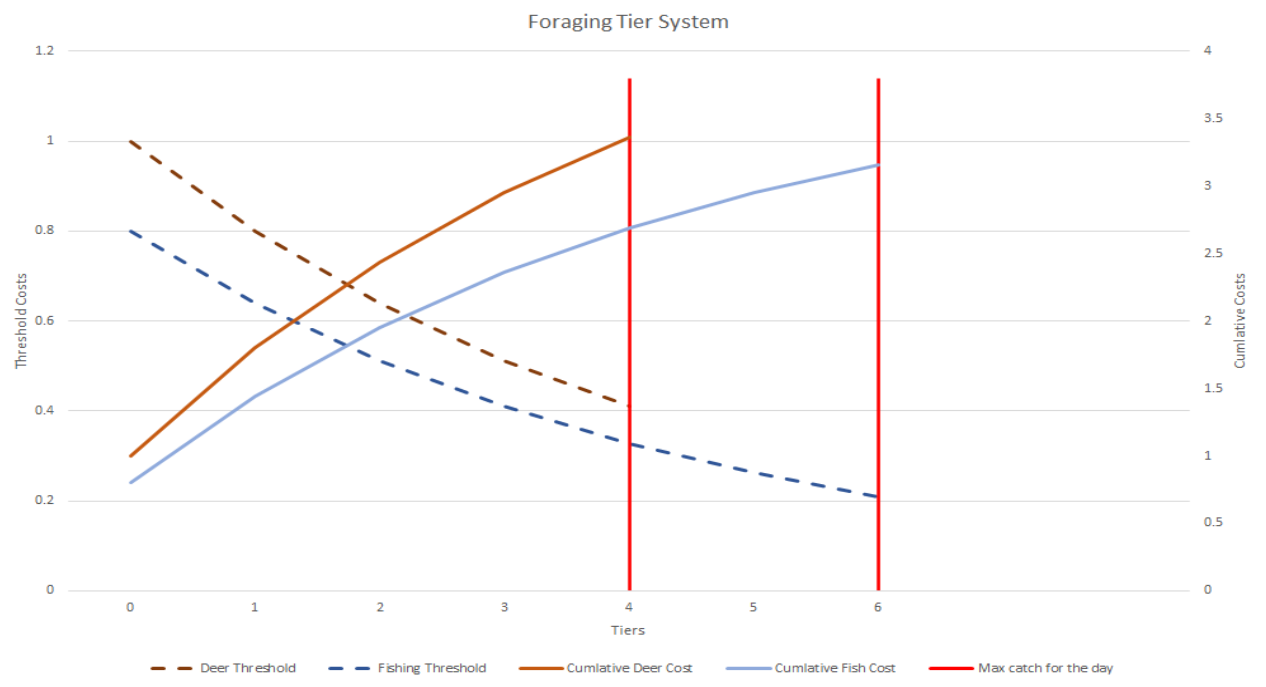
\includegraphics[width=0.6\textwidth]{04_environment/Images/Foraging Tier System.PNG}
    \caption{Foraging Tier System}
    \label{Images:Foraging Tier System}
\end{figure}

As the tiers increase the cost per animal decreases but the total cost increases up to a daily catch limit. Thus if teams collaborate, they could invest less as individuals to get a good return through deer hunting, however if they invest too much then they will over spend as they reach the daily max catch. Thus it would be beneficial for some teams to go fishing which has a higher maximum catch per day but comes with lower returns (thus there is a need for some self sacrifice to be done to reach maximum welfare). \\ 

Fishing has similar functions with the key difference being the Tiers start at 1 and Normal distribution. \\

\subsection{Examples Distributions}
\subsubsection{Example of the distribution for foraging return (Deer hunting - payoff dominant)}

\begin{figure}[!htb]
    \centering
    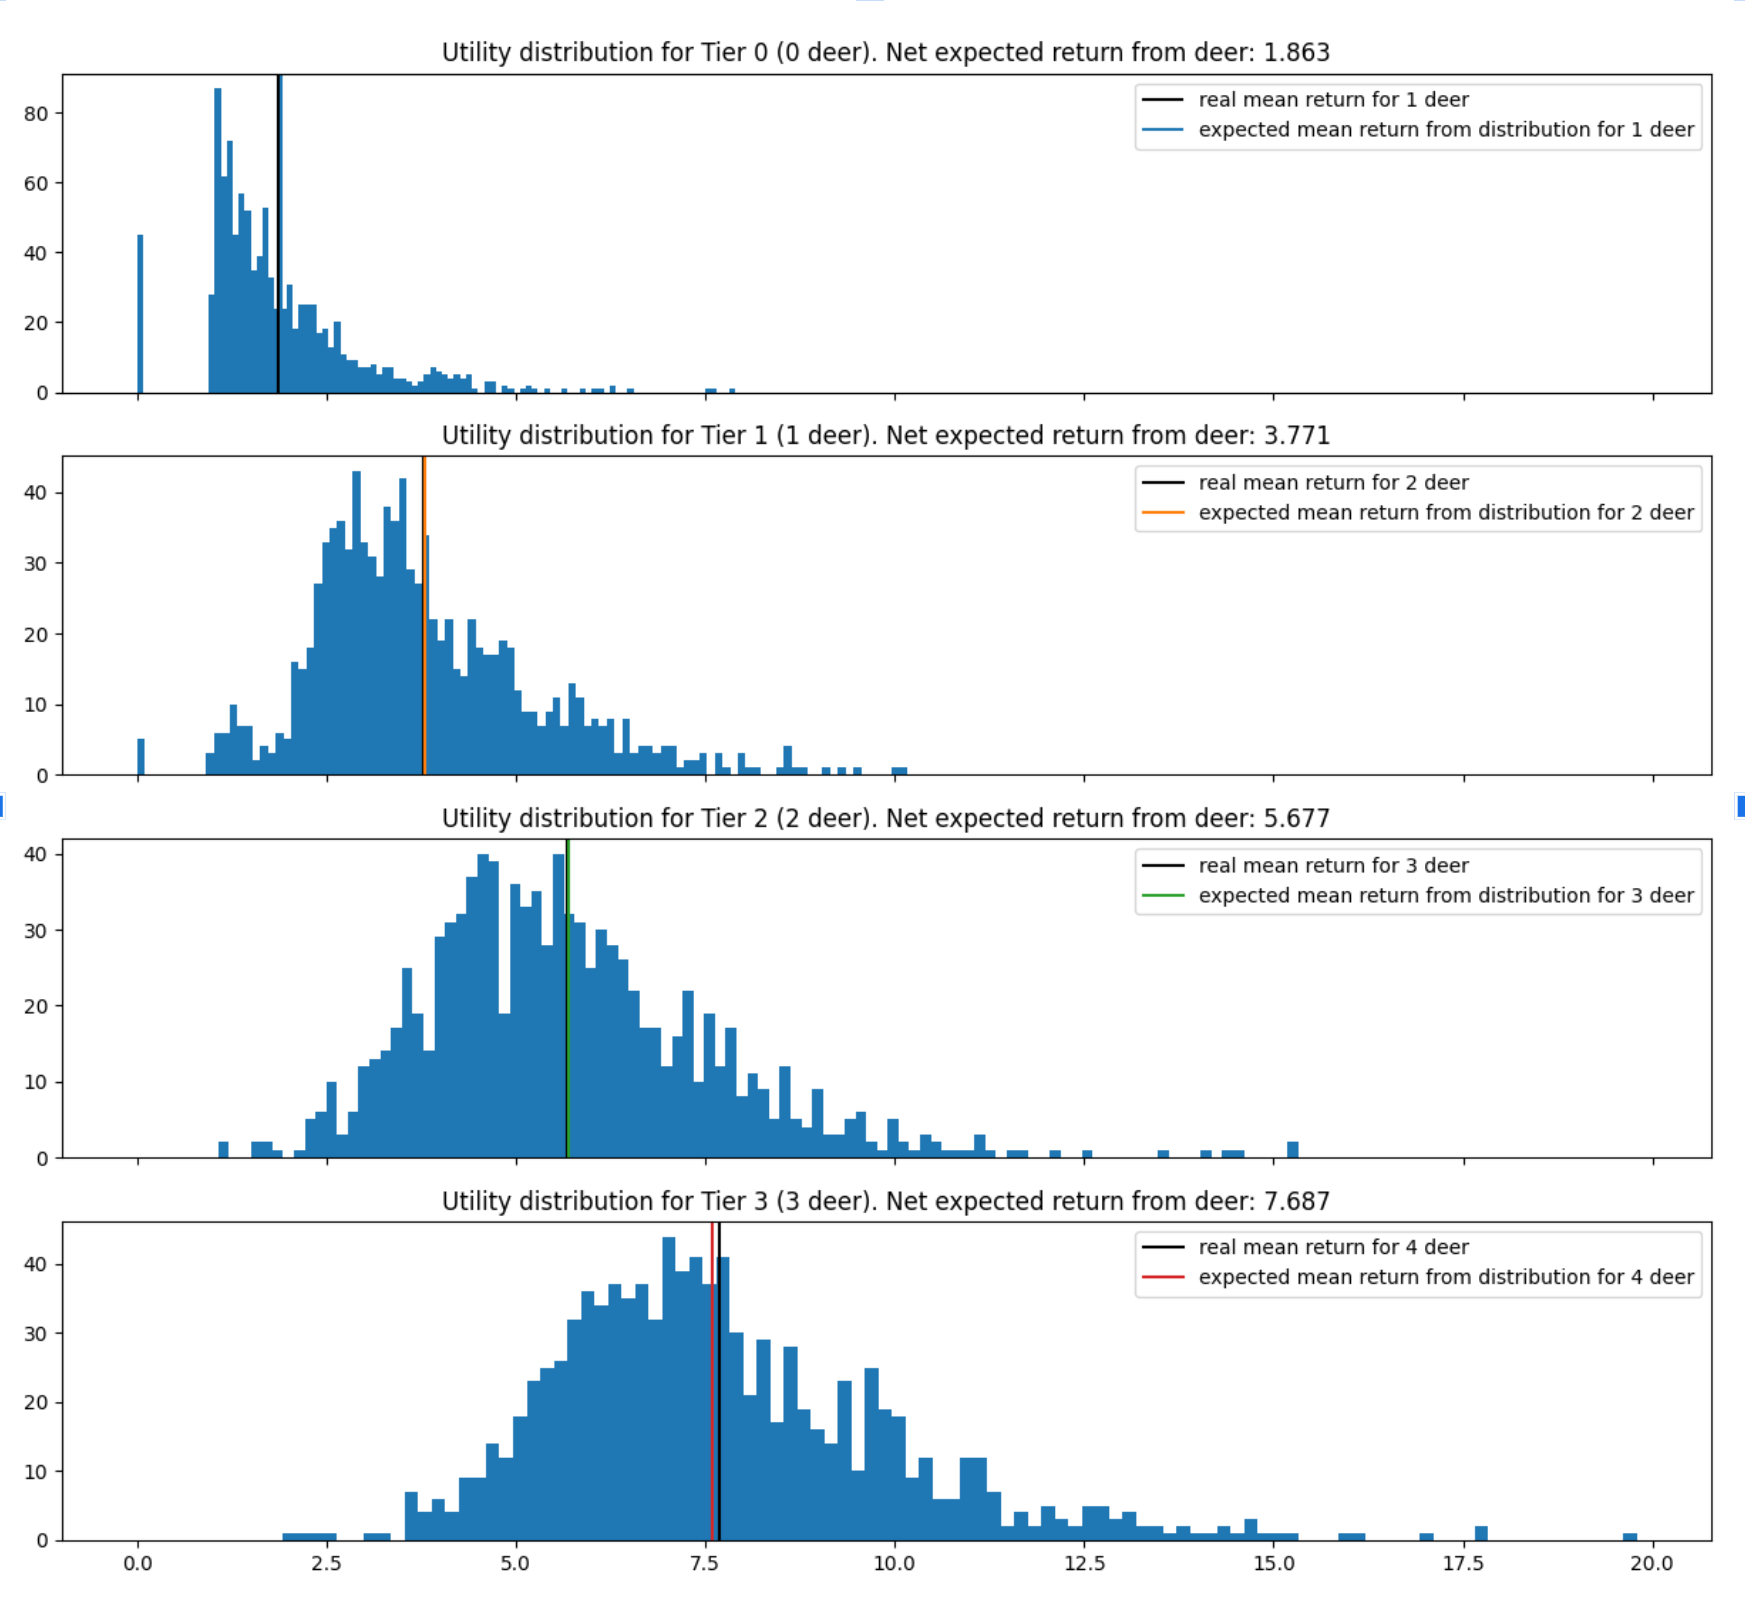
\includegraphics[width=1\textwidth]{04_environment/Images/Distribution of Foraging returns Deer Hunting.PNG}
    \caption{Deer hunting payoff dominant Distribution for foraging return}
    \label{Images:Distribution of Foraging returns Deer Hunting}
\end{figure}

To increase the risk we have used a Bernoulli Random Variable (D) that makes it possible for the hunt to not return any resources. Whilst the Exponential Decay (W) is to disincentive too much resources being placed in hunting and hoping for a high return. However this all comes with the benefit of significantly higher (2x) returns than fishing.\\ 

The above graph represents the return utility which represents the return multiplier of the foraging. The average \textbf{expected mean} return across 1000 iterations is shown by the colourful lines which is close to the \textbd{real mean}. \\

\newpage
\subsubsection{Fish hunting - risk aversion}

Fishing is similar to Deer hunting, except that it uses only a Normal Distribution (F), which focuses on avoiding risk by being very predictable and safe. The Figure below illustrates the return utility function of fishing.\\

\begin{figure}[!htb]
    \centering
    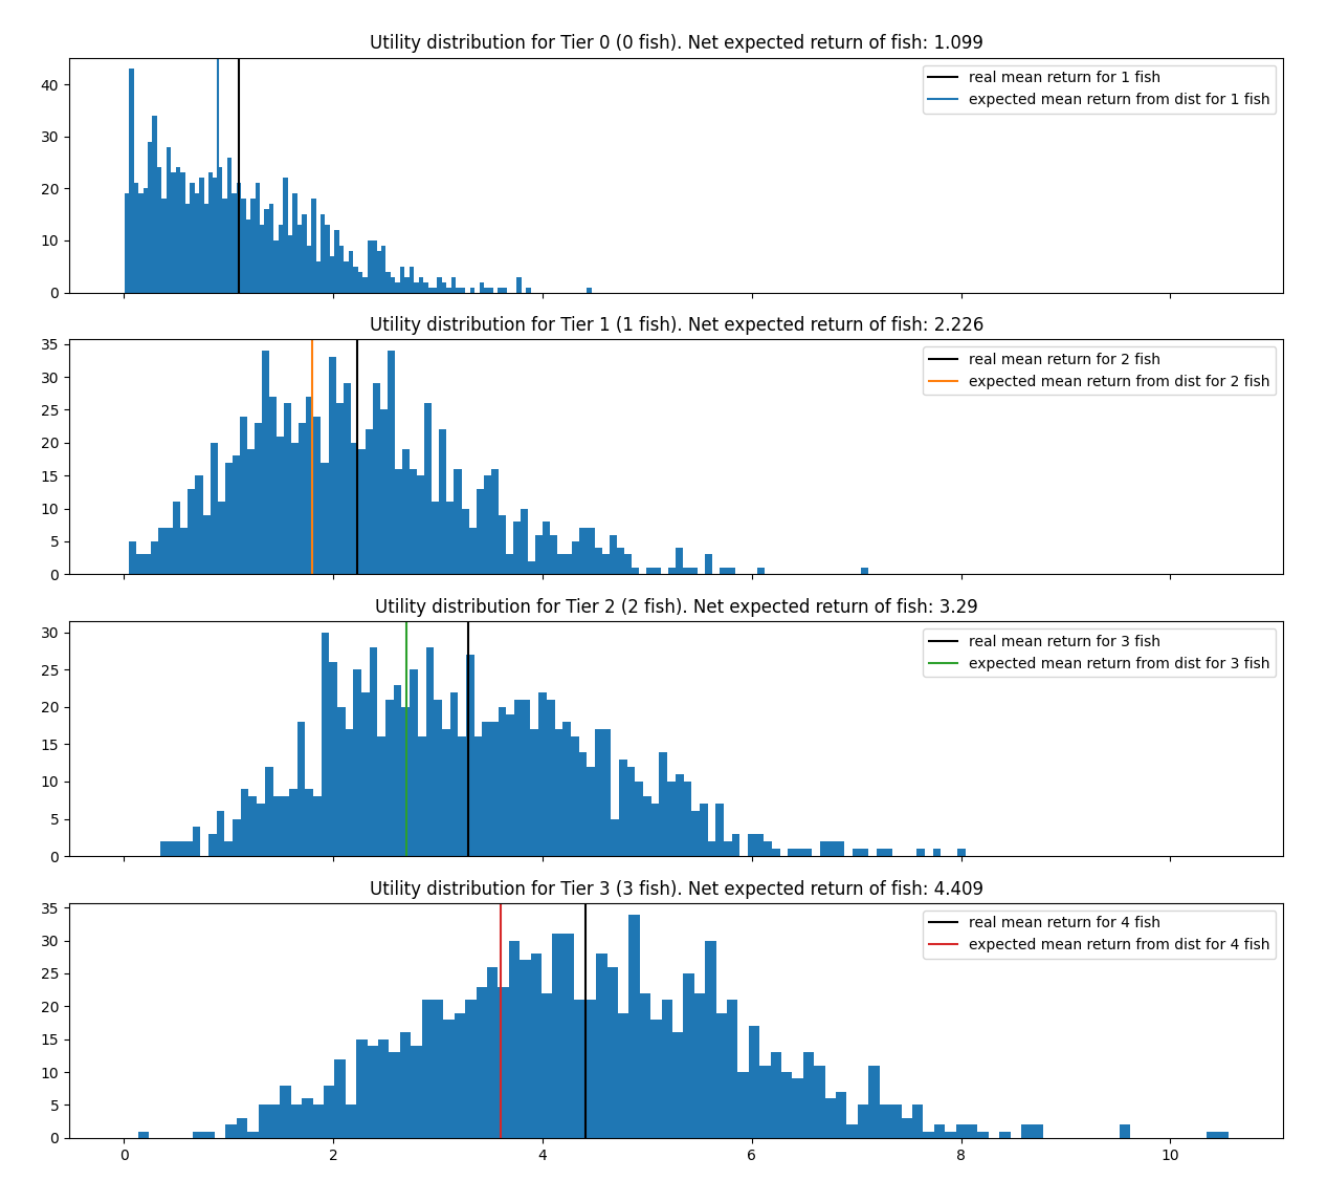
\includegraphics[width=1\textwidth]{04_environment/Images/Distribution of Foraging returns Fishing.PNG}
    \caption{Fishing Risk aversion Distribution for foraging return}
    \label{Images:Distribution of Foraging returns Fishing}
\end{figure}

As seen in the graphs the return for the deer is almost double that of the fish return whilst the fish return is much easier to obtain due to the lower cost of catching fish. \\

\newpage
\subsection{Solution concepts}
\subsubsection{Dominant Strategy}

In our implementation there is no dominant strategy as picking deer hunt when other players switch to fishing could lead to significantly worse returns due to insufficient resources. Whilst picking fish hunt when enough resources are invested in deer hunting will net you a worse return than if you went deer hunting.\\

\subsubsection{Nash Equilibrium}

In the regular stag hunt game there are 2 pure Nash equilibria, where both players go for either payoff or risk aversion. In our implementation there are multiple Nash Equilibria; these would be the points where the islands cannot benefit themselves by moving to deers hunting to generate more return. As there is a limit to how many deers that can be hunted thus by moving to deer hunting they are getting a worse return than if they just stayed at fishing. Whilst the islands at the deer hunt are already making a greater return and have no reason to switch to fishing.\\ 

\subsubsection{Pareto Optimal Strategy}

At some point all players will be in a position where changing foraging methods will not yield any better income for themselves and in fact also hinder others. This is due to the max daily deer hunt limit which will create a maxim return on the deer hunt. Therefore there will be points where the islands will change as the amount of resources being entered into both methods of foraging is the most efficient, this being where deer returns are maximised. There may also be a point where the user can benefit by switching away from deer hunting, however this will cause the other islands in the deer hunt to have a worse pay off due to a possible drop in tier resulting in worse returns.\\

\begin{figure}[!htb]
    \centering
    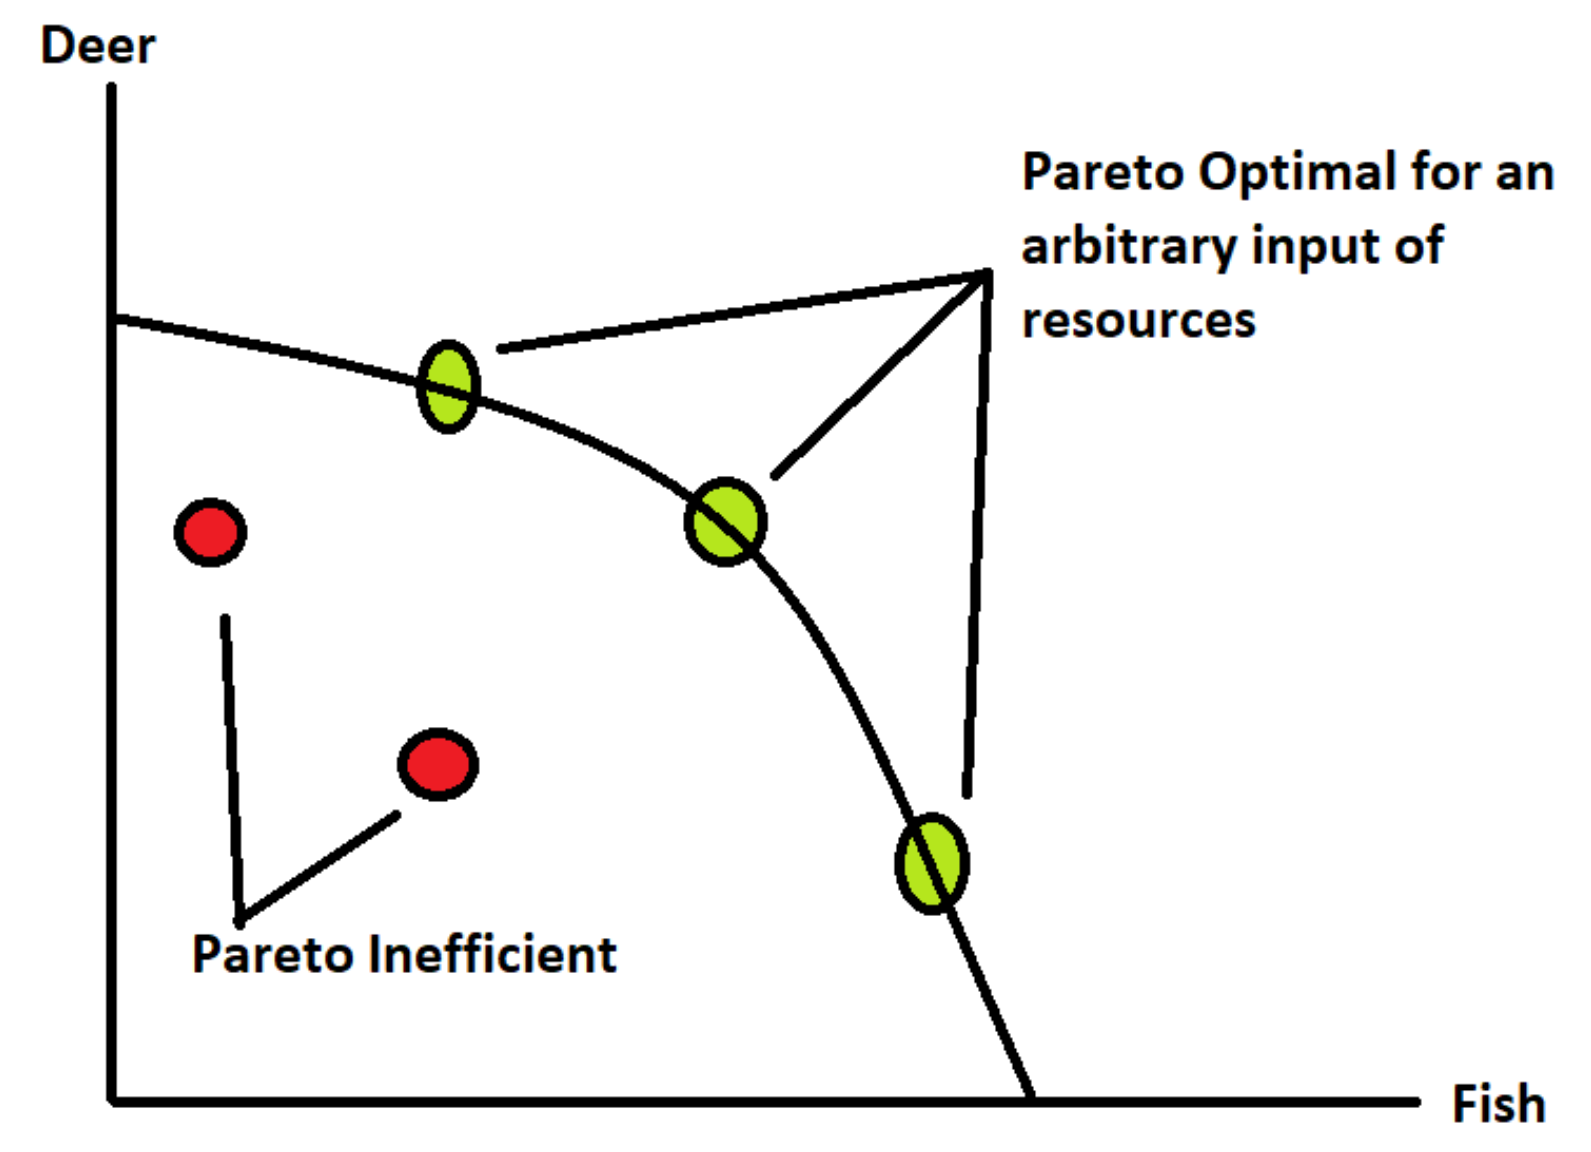
\includegraphics[width=0.7\textwidth]{04_environment/Images/Pareto Optimal Strategy.PNG}
    \caption{Pareto Optimal Strategy}
    \label{Images:Pareto Optimal Strategy}
\end{figure}

\subsubsection{Social Welfare Maximisation}

It is possible for these islands to find the social welfare maximum in this foraging function with enough time. The islands could identify the exact amount of resources needed, for both fishing and deer hunting, to achieve the best return according to the maximum number of animals. Thus by cooperating who goes where and spends how much they are able to maximize their returns without spending more resources than necessary.\\

\subsection{Post-MVP Extended Work}

For the post-MVP implementations, our additions focus on further exploring the dynamics of our agents and allowing for a more complex decision-making interaction between clients and the environment. Some of these design ideas were implemented in the post-MVP self-organising multi-agent system and others are expressed for the sake of completeness and future work recommendations.\\

Some changes have been made to make foraging more volatile and unpredictable. These will add to the complexity of the system, allowing the teams to further evaluate the clients’ performance on observing and using learned knowledge to take action.\\

\subsubsection{Incorporated Changes: Population density}

Introducing a model that controls the population density of deer allows us to increase the complexity of the foraging function. In short, the deer hunting capacity decreases with decreasing population and increases with an increasing population. This will then influence the maximum deer per hunt parameter(n), which in turn results in a more complex return calculation function (\textbf{DtotalReturn}), which would make it harder for agents to figure out forage tier boundaries to optimise their strategies.\\

The population change can be dynamic depending on various environmental factors, fetched from the rest of the system. For example, a Disaster could supposedly cause the population density of deer to halve, making it harder to forage and therefore, causing lower returns. For the post-MVP implementation, the team uses a single species population model and more specifically logistic modelling for the deer and fish population. The model can be described in the equation below. \\

\begin{equation}
\frac{\mathrm{d} P}{\mathrm{~d} t}=k(N-P)
\end{equation}

\begin{itemize}
        \item “P” is the total Population \item “N” is the maximum deer/fish population (“carrying capacity” formally)
        \item “k” is the growth coefficient
        \item “t” is time
    \end{itemize}

In our implementation \textbf{“k”} and \textbf{“N”} are constants but it would be interesting to see what would happen if we were to increase the growth coefficient, causing a population growth and observing the islands’ dynamics. Will they keep on “investing” higher resources each turn, taking advantage of the deer/fish abundance, or will they stick to their original, safe and static strategy?\\

Below, we can see a simulation of the implemented logistic model, with a growth coefficient of 0.2 and \textbf{“N”} of 8. It can be seen that overtime there is an unpredictable pattern to population changes, which would be interesting to see affecting the tier system and in extend, the deer/fish foraging strategies of the agents.\\

\begin{figure}[!htb]
    \centering
    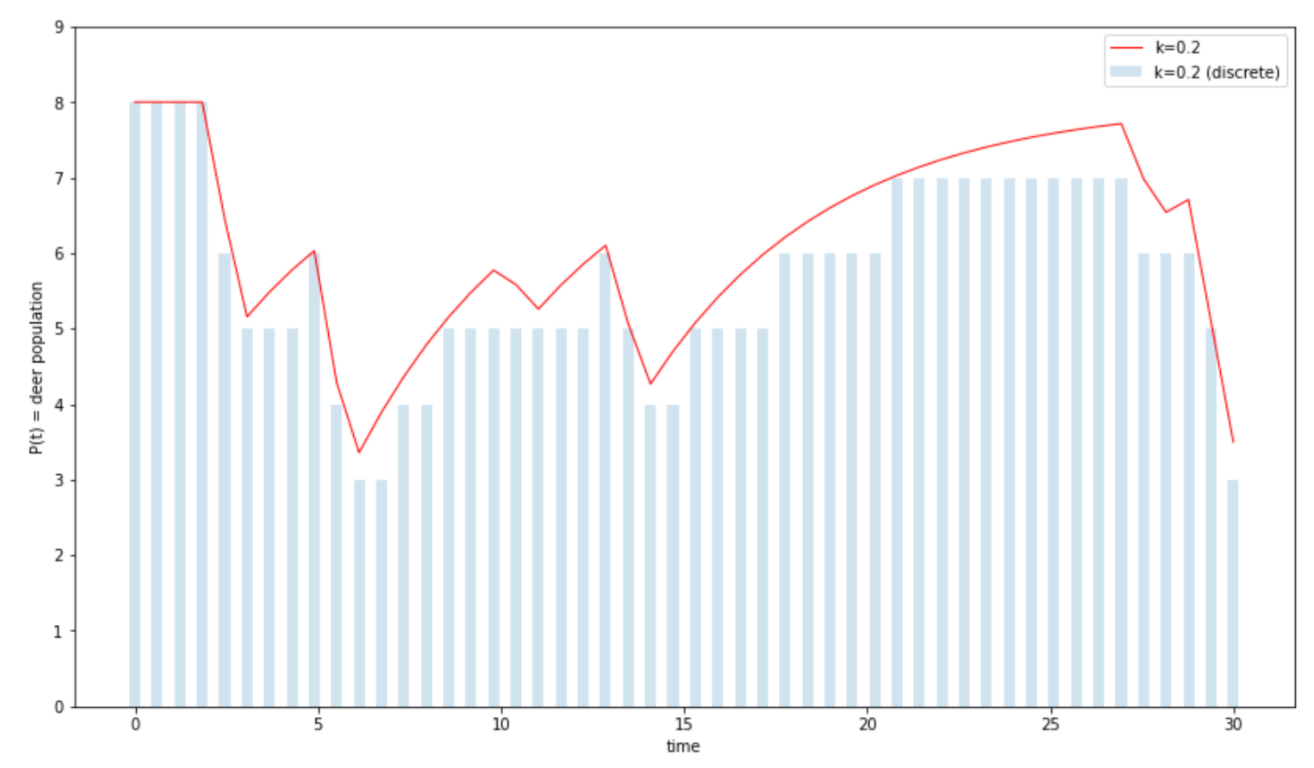
\includegraphics[width=1\textwidth]{04_environment/Images/Deer population over time.PNG}
    \caption{Deer population over time (turns) under Logistic modelling with a growth coefficient of 0.2.}
    \label{Images:Deer population over time}
\end{figure}

Modelling the population (or linking it to other environmental elements) allows us to make sure that the system’s dynamics are varying, making it harder for islands to settle onto a single foraging method because it always results in better returns. Pareto optimality is therefore harder to achieve and thus maximising social welfare is trickier, requiring agents to make more informed decisions, recognizing possible patterns. Of course, that would be an easier task for the islands, if they had knowledge on what is affecting the population (i.e. disasters), whereas a logistic model function might be more abstract in the eyes of our agents, requiring more processing. \\

\subsubsection{ Incorporated Changes: Method of resource allocation}

Lastly, in the post-MVP implementation, a parameter can be set that allows either an equal split of returns after foraging no matter the input, or a proportional split that is dependent on the amount of resources inputted by each island. Both of these implementations work in accordance to the previous specification. Such change will allow us to observe the concept of free-riding further, looking at how greedy islands behave in the case of uniform resource returns. Will the islands seek to minimise inputs and benefit from the more generous islands, even at the cost of being allocated a lower tier? Will they input just enough to maximise the tier they are foraging in? Or, will they observe other island’s previous contributions and make a decision based on that? These are some of the questions we can explore using this post-MVP change. \\

\subsection{Future Work Concepts}

Further work could be done to make sure that there is enough complexity to explore the dynamics of our agents. Due to the project’s time constraints, some interesting ideas were not implemented but were thoroughly examined during the design process.\\

An important add-on to our previous implementation could be the enforcement of laws by the IIGO for the number of islands that can go foraging. That would introduce the need of internal client relationships, adding another level of decision-making complexity to the agents. The specific alteration could result in some interesting findings. For example, there could be an auction scenario where islands would bid with their input resources, where only the highest bidders would be able to forage, as limited by the IIGO. Therefore, Islands with the lowest resources would be out-bidded, possibly causing a long-term resource depletion that would need to be mitigated by the more resourceful islands later in the game. It would be interesting to see how such change would affect the free-rider problem and how islands would adjust their strategies to out-bid other islands.\\

Another change that could be made, is to let islands choose who they can forage with. That could be in the form of direct messaging or voting. Essentially, our speculation is that agents would avoid the free-riding problem in both cases by enabling agents to make collective decisions based on communicated resource contributions. That’s because free-riders would be out-voted or not invited for foraging. That, in combination with the aforementioned tier system, would possibly result in all the islands contributing as much as possible to the input foraging “pool”.  However, it would be interesting to see if islands can then reach Pareto optimality, where every single agent gets the best possible return for their input.\\

In addition to the above suggestions, area limited foraging where agents would only be allowed to forage with only one neighbouring island using a ranking algorithm. This could also be enforced and implemented in a future iteration. Moreover, this particular scenario could be extended by programming prey densities to be geofocused, where prey populations could vary between regions on the “map”. Islands would then need to make a strategic plan on how their ranking of neighbouring islands would change in accordance to their returns and returns broadcasted from other island pairs.\\

Finally, more foraging options could be added in future implementations. For example, a third foraging technique, call it whale it hunting, could be created. That would have an even higher return than the deer hunting, deeming it an appealing forage method. The barriers of entry could be similar to that of the deer hunting method in this scenario but at the same time, there would be a more spaced out/expensive tier system. This combination would potentially incentivise cooperation between islands, if their strategy was to maximise returns. Also, as we have introduced more foraging methods, it could be the case that we hard-fix the type of return for each method and observe how agents decide to behave. For example, we could have the deer and fish hunting methods result in returns proportional to inputs, whereas the whale hunting method would result in an equal split of returns between all participating islands. Would this mean that islands choose a fairer division of returns and not go on whale foraging at all? Or Would they be intrigued by the higher costs and choose whale hunting over the other foraging methods? In the latter question agents would need to take in mind that an island may be entering an insignificant amount reaping however, a large reward. It is therefore up to the islands to decide if the higher payoff is worth the risk of other islands free-riding.\\

All of the aforementioned behaviours are of course influenced by island tactics and therefore, an island programmed to be greedy will not cease to be greedy no matter how the surrounding islands’ behaviours change, unless the greedy island can adapt. Therefore, conclusions drawn on specific foraging methods, and how agents react with them, need to take this into account.\\

\newpage
\section{Disaster}
\subsection{Disaster Background}

A game has been designed, where agents are at risk, they will be directly confronting a risk/a disaster once every round. This subset of the game creates a dilemma, where each island (agent) has to survive. They will have the opportunity to work together by investing collectively to the common pool, the disaster will be mitigated if the islands invest enough resources to reach a desired threshold. Otherwise, the islands would face negative impact, which would diminish their available resources. It is worth mentioning that the disaster will first extract resources from the common pool, and then if not enough resources have been invested, resources will be depleted from each island proportionally to their island’s damage.\\

Furthermore, the disaster has been designed to comprise of an epicentre (eye of the storm), which is limited within the archipelago bounds, it is represented using Cartesian coordinates (EpiX, EpiY). Therefore, all islands or a subset of islands may be affected due to their proximity to the disaster epicentre. The island’s proximity to the disaster epicentre is directly proportional to the island’s damage. In other words, the island's available resources will be diminished based on the disaster magnitude and its location with respect to each island’s fixed location.\\

The following example can briefly explain the dilemma:\\

The closest an island from the eye of the storm, the larger the severity on that island. Therefore, the more resources are depleted. Let’s say that the disaster epicentre hits around island 1 as shown in Figure below. and that the desired common pool threshold has not been met. Island 1 would be experiencing severe damages , and island 2 and 6 some damages and the other islands low to no damage. Therefore, Island 1,2 and 6 have the risk of not surviving if they are lacking resources, whereas island 3, 4, and 5 would not be affected as much by the disaster.

\begin{figure}[!htb]
    \centering
    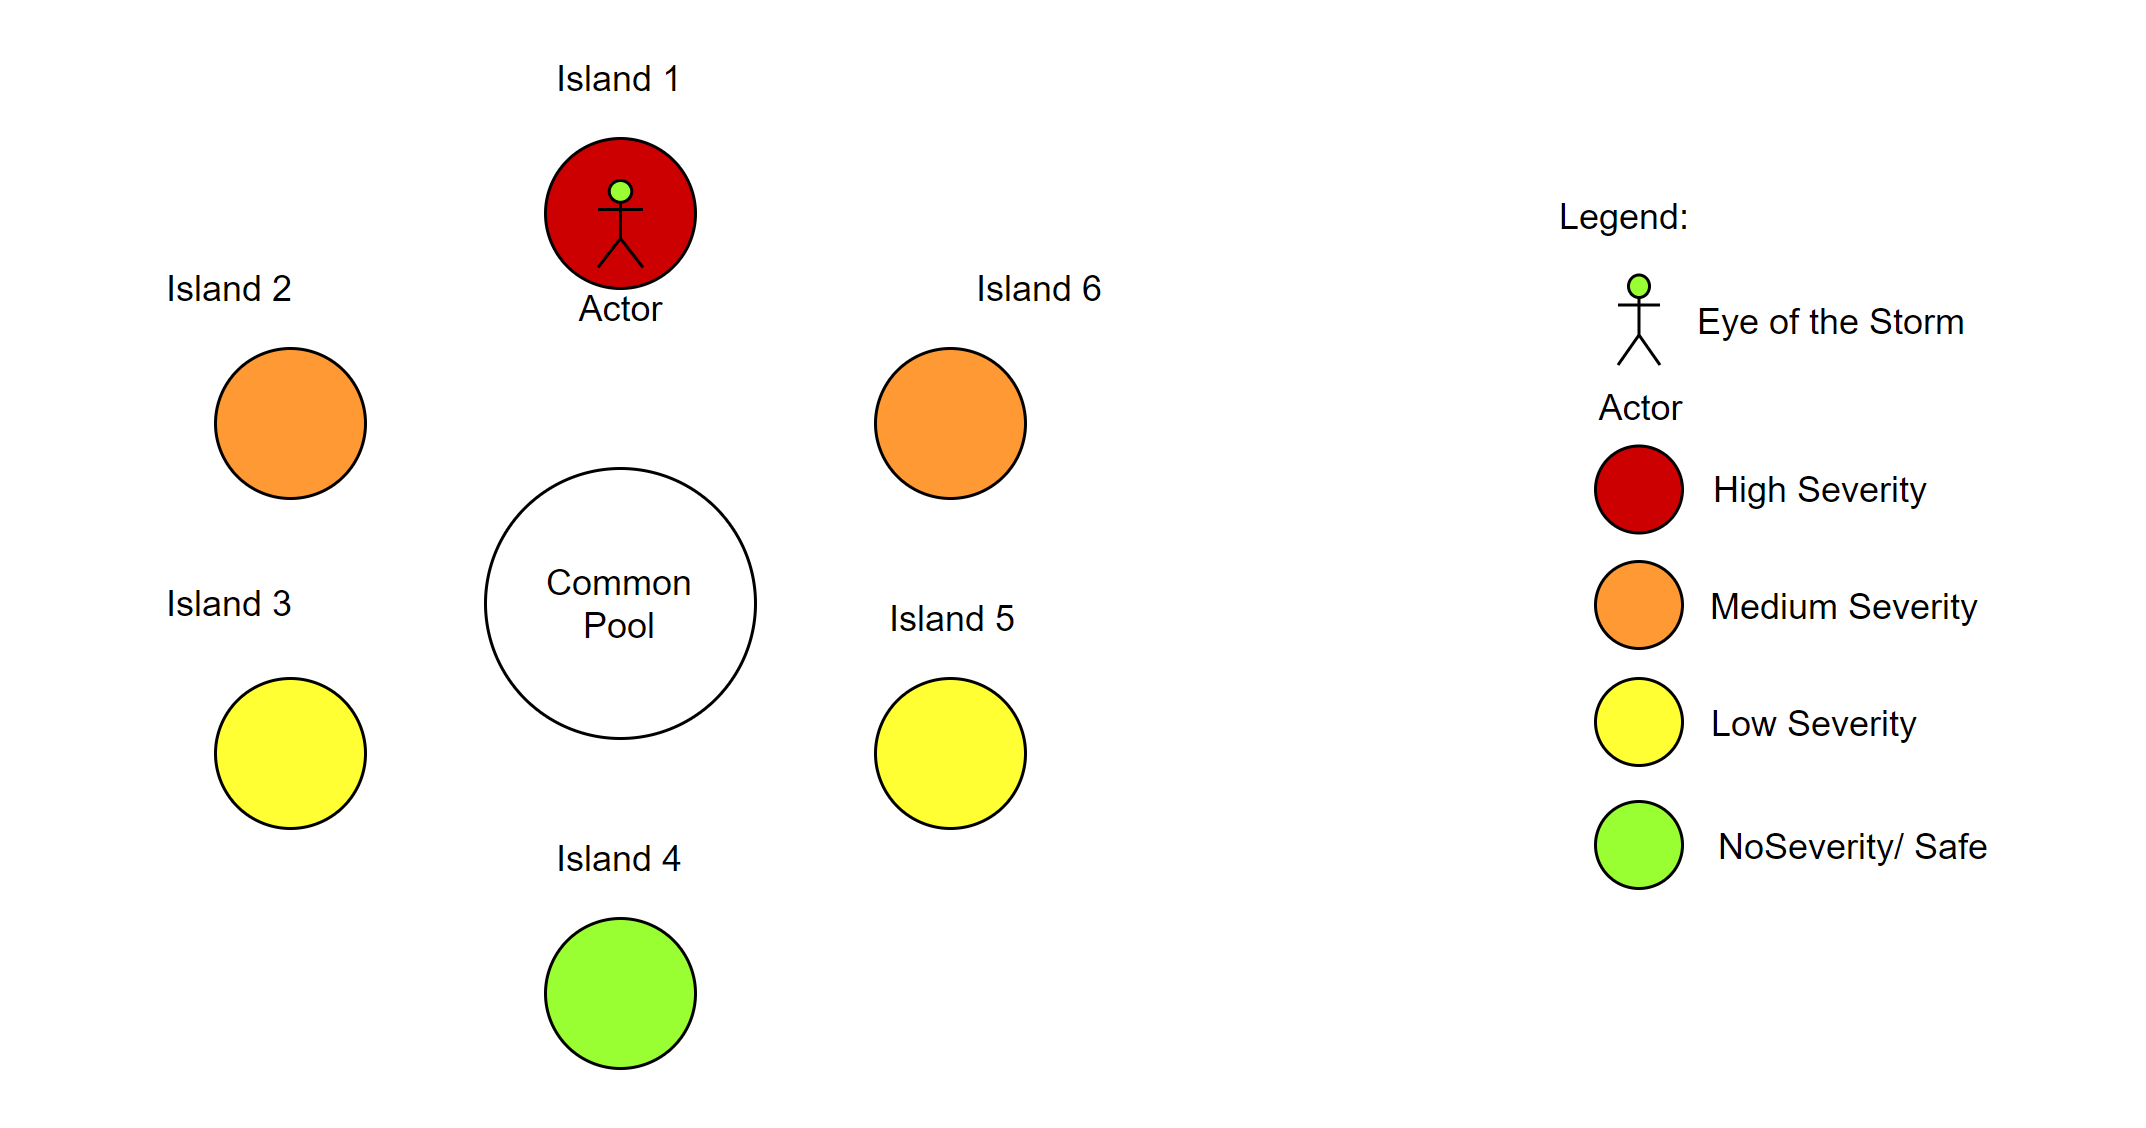
\includegraphics[width=1\textwidth]{04_environment/Images/Disaster eye of the storm severity.PNG}
    \caption{Disaster Epicenter effects}
    \label{Images:Disaster eye of the storm severity}
\end{figure}

\newpage
\subsection{MVP Functions within the Disaster}
It is worth mentioning that the island's geography in infrastructure is the combination of the island number and the island’s fixed location in the archipelago.\\

\begin{table}[h]
\begin{center}
\begin{tabular}{|p{1.1in}|p{1.1in}|p{1.1in}|p{1.1in}|} \hline
\textbf{Functions} & \textbf{Description} & \textbf{Inputs} & \textbf{Outputs} \\ \hline
\textit{Bernouilli Distribution (pdfGlobal)} & Whether a disaster is going to occur & -The probability of a disaster occurring,\newline -The Global probability variable & Determines the likelihood of a disaster occurring \\ \hline
\textit{PdfMag} & Exponential distribution & -The spatial PDF & Determine the disaster magnitude \\ \hline
\textit{Epix,Epi Y} & Spatial probability distribution function & -The spatial PDF\newline -Disaster Magnitude & Determines the location of the disaster epicentre \\ \hline
\textit{DisasterEffect} & Island's Proximity distance to the eye of the storm & -Island geography\newline -Eye of the storm location & Determine the islands damage \\ \hline
\end{tabular}
\caption{\label{tab:table-name}Disaster's main functions}
\end{center}
\end{table}

The disaster has been computed as part of the infrastructure: Each island has a fixed position, characterised using Cartesian coordinates. They are located in the archipelago which captures the collection of island geographies including the bounding regions of the entire archipelago.\\

Furthermore, to determine when a disaster is going to occur, we have used the Bernoulli random variable (probability of a disaster occurring is low).\\

The Spatial probability distribution function "Spatial PDF" is uniform and it controls the distribution works of XY grid of the location of the disaster. The magnitude is then exponentially distributed (it exponentially more likely to have a smaller magnitude as we want large disasters to be more rare, occur less frequently). In addition, we have created a magnitude variable "Lambda" which can vary the slope of the exponential function (create a harsher environment when increasing the "lambda variable" by creating larger disasters and vice versa). In addition, the eye of the storm (disaster epicentre) is limited within the bounds of the environment (The environment bounds are fixed, they are specified by the users).\\

\begin{figure}[!htb]
    \centering
    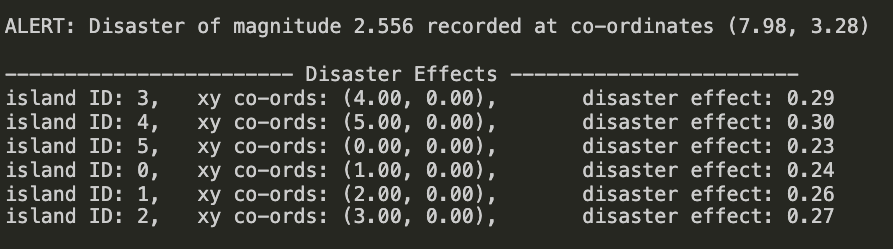
\includegraphics[width=1\textwidth]{04_environment/Images/Disaster output infrastructure.png}
    \caption{Infrastructure Disaster outcome}
    \label{Images:Disaster output infrastructure}
\end{figure}

The image above illustrates the output of the disaster, it first shows the magnitude of the disaster and the precise location of the eye of the storm, it indicates as well the fixed location of each island as well as the proportional effect of each island. For example, Island 2 with a fixed location of (5,0) has the largest disaster effect, which means it is the closest to the eye of the storm.\\

\subsection{Future works Concepts}

For the MVP, the disaster is a random function, meaning that it is possible to predict it with the current game.\\

There are multiple future works ideas that would be developed in the design aspect such as; a deterministic disaster which would be  designed as a straight line that accumulates during the days, once the threshold has been met then the disaster would occur. Another deterministic disaster idea would be to link the disaster’s magnitude to time. Thus, agents will have to learn from past disaster occurrences, creating a memory. Agents will start learning from past disasters and will be able to forecast the next one. Therefore, the agents will be able to forecast that if a disaster did not surface for a long period of time, then the magnitude of the next disaster will be much larger than the previous one.\\

Another Idea is that agents can invest into forecasting. Therefore, agents will have access to a history of past disasters, which would be utilised by the agents to learn and gain knowledge in order to predict the upcoming disaster. The larger the amount of resources invested; the agents will have access to a larger history of previous disasters. Therefore, agents will acquire knowledge, when investing resources.\\

\section{Common Pool}
\subsection{Common Pool Background}

We are designing a game where 6-islands (agents) are having access to a common-pool resource. In micro-level, each island intends to maximise its utility while in macro-level, all the islands want to maintain sustainability and be protected by the upcoming disaster. The above description specifies a collective action problem where n-agents (6 in our case) are seeking access to a common pool resource that is sufficient to satisfy some agents but not to satisfy all of them.\\

We have implemented a Linear Public Goods (LPG) Game where all the agents individually own some resources and try to maintain and increase them, by foraging, but also contribute a part of them to the common pool. This common pool is used for the payment of expenses of the institutional roles and for the protection towards the disaster.\\

In more detail, the common pool is represented by a structure with following characteristics:

\begin{itemize}
    \item Common Pool Threshold
    \item Amount of Resources 
\end{itemize}

According to the specifications of an LPG Game, the agents should be able to perform the following actions:  

\begin{itemize}
    \item Request Resource from the Common Pool 
    \item Contribute Resource to the Common Pool 
\end{itemize}

And the Common Pool is responsible for two more actions: 

\begin{itemize}
    \item Mitigate Disaster
    \item Deplete islands after a disaster
\end{itemize}

\newpage
\subsection{MVP functions within the Common pool}

For each of these action a relevant function has been implemented as follows:\\

\begin{table}[h]
\begin{center}
\begin{tabular}
{|p{1.1in}|p{1.1in}|p{1.1in}|p{1.1in}|} \hline
\textbf{Name} & \textbf{Description} & \textbf{Input} & \textbf{Outcome} \\ \hline
\textit{islandDistribute} & Distribute Resources from Common Pool to Island upon Request & -Requested Amount of Resources\newline -Island Name & Resources subtracted from CP and added to island \\ \hline
\textit{islandContribute} & Contribute Resources from Island to Common Pool & -Donated Amount of Resources\newline -Island Name & Resources subtracted from Island and added to CP \\ \hline
\textit{DisasterMitigate} & Mitigate the Disaster with the Amount of Resources in the Common Pool & - Effect of Disaster to each island\newline - Proportional effect of Disaster to each island (magnitude of disaster divided by the distance of the island from epicenter) & Resources in CP were exploited for the mitigation of the disaster and remaining effect has to be mitigated by each island \\ \hline
\textit{islandDeplete} & Deplete Islands after the disaster (with the amount of disaster that couldn't be mitigated by CP) & -Remaining effect for each Island\newline -List of Islands & The remaining proportional effect of the disaster to each island is causing the depletion of resources \\ \hline
\end{tabular}
\caption{\label{tab:table-name}Common Pool's main functions}
\end{center}
\end{table}

The common pool has been computed as part of the infrastructure: with a threshold that is the amount of resources to hopefully help to completely mitigate the disaster. If the threshold is met, the damage from the disaster on the common pool and islands will be half the actual amount. This incentivises islands to contribute to the common pool and reflect the reality that, if there is enough preparation for the disaster, the damage will be much less compared to no preparation. In the MVP, the threshold is a fixed value.\\

Another important input to the implementation is the magnitude of the disaster’s damage to each island. As shown in Figure 1.8 , the disaster’s magnitude is 3.458. However, the disaster’s effect on individual islands do not add up to 3.458 because the storm’s epicenter is further away from the islands. This aspect creates a more realistic scenario to the game. From the islands’ individual damage, proportional effects are calculated to determine which island has been hit harder out of the 6 islands. The summation of these proportional effects is equal to 100\%, which is the total effective damage. \\

If the common pool has enough resources to fully mitigate the disaster, the process is very easy. However, in the unfortunate events, the common pool resources will be used to mitigate each island's damage according to their proportional effect i.e., if an island is hit harder, it will receive more help from the common pool. This is also visualized in Figure 1.8, as island 4 withstands most damage from the storm, the common pool gave island 4 most help with 252.47 resources (“common pool mitigated” column). The updated damage value shows the leftover damage of the disaster that the common pool was not able to mitigate. These leftover damage will be used to further deplete the island's private pool of resources. If there are enough resources in the common pool totally mitigate the disaster then the update damage values will be 0.\\

\begin{figure}[!htb]
    \centering
    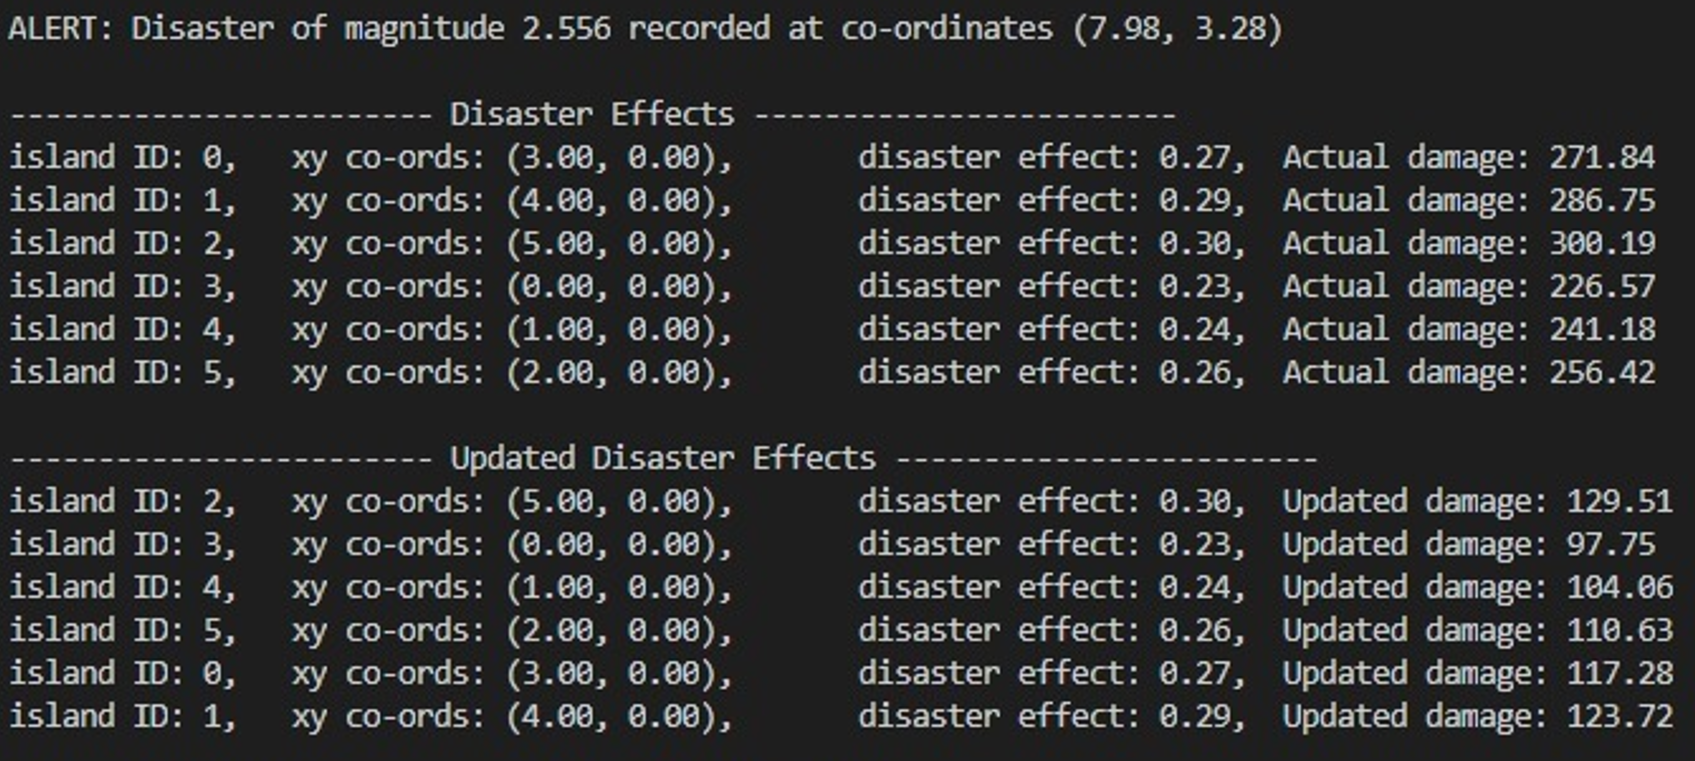
\includegraphics[width=1\textwidth]{04_environment/Images/Common Pool infrastructure outcome.PNG}
    \caption{Demonstration of how common pool works in software}
    \label{Images:Common Pool infrastructure outcome}
\end{figure}

For the MVP, the common pool threshold is a fixed value and known to islands. In the post-MVP, the functionality of making the Threshold unknown to the islands would be added. \\

The common pool resources will be given to each island based on the severity of the damages.\\

If the amount of resources in the common pool exceeds the total effect of disaster, then the leftover amount of resources in the common pool will be used for the next round.\\

Since the goal of each island is to maximise its utility, the following dilemma shows up: islands can free ride by not contributing to the common pool and yet receiving the benefits after a disaster or if they are aware that they would not be depleted by the disaster - since they are far away from the eye of the storm - they might also not contribute to the common pool and thus the rest of the islands would be severely destroyed. \\

The following example can briefly explain this dilemma:\\

If the epicentre of disaster is known to the islands and happens to coincide with the location of Island 1, then Island 4 might not contribute at all to the CP since it will not be affected by the disaster. Moreover, Islands 3 and 5 that will not be severely hit might contribute a small amount to the CP or even zero amount (free riding case). Since the rest of the islands might contribute to the CP, then Islands 3 and 5 will be profited by the contribution of others.\\

We wanted to highlight the importance of prevention and incentivise islands to contribute to the CP, thus if the amount of resources in the common pool exceeds the threshold when the disaster happens, then the “power” of disaster towards the islands and common pool will be decreased. It makes sense in real life, as more preparation will result in less damage. For the MVP, the actual damage of disaster is decreased by half, but this can vary in the post-MVP.\\

\subsection{Example distribution}
This can be described by the examples in table X, which shows 4 possible scenario:\\ 

\begin{itemize}
    \item Contribution to common pool does not meet threshold and common pool cannot fully mitigate disaster’s damage
    \item Contribution to common pool does not meet threshold but common pool can fully mitigate disaster’s damage
    \item Contribution to common pool meets threshold but common pool cannot fully mitigate disaster’s damage
    \item Contribution to common pool meets threshold and common pool can fully mitigate disaster’s damage
\end{itemize}

\begin{table}[h]
\begin{center} 
\begin{tabular}{|p{0.9in}|p{0.9in}|p{0.9in}|p{0.9in}|p{0.9in}|} \hline
& \textbf{Scenario 1} & \textbf{Scenario 2} & \textbf{Scenario 3} & \textbf{Scenario 4} \\ \hline
\textbf{Disaster total damage} & 1000 & 200 & 1200 & 1200 \\ \hline
\textbf{CP's threshold} & 500 & 500 & 500 & 500 \\ \hline
\textbf{CP's current value} & 300 & 300 & 500 & 700 \\ \hline
\textbf{CP's multiplier} & 1 & 1 & 0.5 & 0.5 \\ \hline
\textbf{Mitigated damage} & 300 & 200 & 500 & 1200 \\ \hline
\textbf{Remaining damage} & 700 & 0 & 100 & 0 \\ \hline
\textbf{CP's remaining value} & 0 & 100 & 0 & 100 \\ \hline
\end{tabular}
\caption{\label{tab:table-name}Demonstration of how common works in different scenarios}
\end{center} 
\end{table}

In scenario 1, the disaster total damage is high, however there is no preparation from the islands through contribution to the common pool. As a result, the common pool could not mitigate all of the damage and 70\% of the damage will be directly on the islands\\

In scenario 2, even though there is no preparation, the common pool is still able to mitigate all of the damage thanks to the low damage of disaster. The leftover resource in the common pool will stay there.\\

In scenario 3, the disaster damage is high. Fortunately, the islands have prepared themselves moderately through contribution to the common pool. Thus, the islands only have to take very little leftover damage.\\

In scenario 4, the disaster damage is high and the islands have prepared themselves very well. As a result, the damage is fully mitigated by the common pool and there is still leftover resource in the pool. 


\subsection{Future Works Concepts}
To observe behaviors of agents in different settings, the future works of the common pool will be centered around varying the values of different parameters such as threshold and threshold multiplier. The forecasting function of the disaster part can be used as a tool to variate the common pool’s threshold and multiplier accordingly. In events that damage could be high, the preparation should be done more carefully, thus the common pool’s threshold can be raised to let islands know about potential damage from disaster. The same thing can be done for threshold multiplier, where the multiplier will be greater for bigger disaster. Since threshold and multiplier both encourage the preparation for disaster, one of them can be fixed at certain seasons to observe different behavior of agents when it comes to varying different parameters. 
